\documentclass[a4paper,12pt,fleqn]{article}
\usepackage{fixltx2e}
\usepackage[utf8]{inputenc}
\usepackage{graphicx}
\usepackage{sidecap}
\usepackage{fancyhdr}
\usepackage{amssymb,amsmath}
\usepackage[swedish]{babel}
\usepackage[margin=1.5in]{geometry}
\usepackage{abstract}
\usepackage[parfill]{parskip}
\usepackage{tocloft}
\usepackage{adjustbox}
\usepackage{textcomp}
\usepackage[T1]{fontenc}
\usepackage{listings}
\usepackage{xcolor,colortbl}
\usepackage{hyperref}
\usepackage{mcode}
\usepackage{a4wide}
\usepackage{caption}

\begin{document}

\section{Inledning}

Vid kommunikation används ofta I-/Q-modulering för att överföra en signal inom ett givet frekvensutrymme. I och med överföringen kan tidsfördröjningar införas. I mottagaränden måste dessa tidsfördröjningar kompenseras för innan överföringen sedan kan I-/Q-demoduleras för att extrahera ljudinformationen 

\subsection{Syfte}

Syftet med denna laboration är att finna bärfrekvens för en given signal, filtrera bort oönskade delar av överföringen och sedan I-/Q-demodulera signalen för att extrahera relevant information. 

\subsection{Materiel och förutsättningar}

Filen signal-hanel742.wav är given med den kända samplingsfrekvensen 400 kHz. Givet är också att filen innehåller en smalbandig signal som är I-/Q-modulerad och har skickats genom filtret nedan. 

\begin{gather}
h(t) = \delta(t - \tau_1) + \delta(t - \tau_2)
\label{equ:filter}
\end{gather}

På förhand ges också att bärfrekvensen för relevant del av signalen är en multipel av 19 kHz.

Signalen innehåller två melodier samt två olika ordspråk. 

För att utföra laborationen används GNU Octave med vertygslådor för ljud samt signaler (octave-audio och octave-signal) installerat. 

% -------- Metod ------------
\newpage

\section{Metod}

Jag börjar med att läsa in filen i Octave och sedan fouriertransformera signalen för att få ut dess frekvensspektra: 

\begin{figure}[htp]
  \begin{center}
  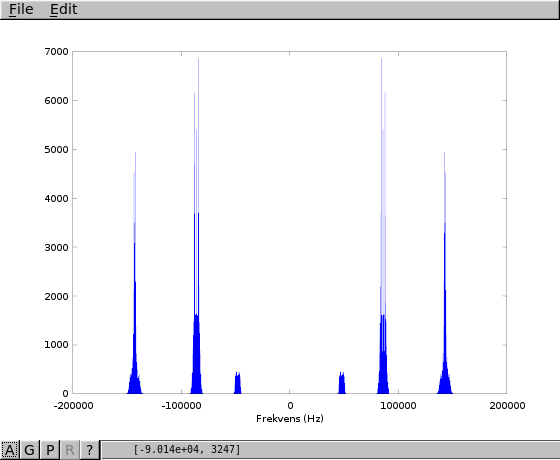
\includegraphics[keepaspectratio=true,width=\linewidth]{fft_orig_data.png}  %skala och filnamn. 
  \end{center}
  \caption{Dubbelsidigt amplitudspektrum för ursprunglig signal} %figurtext.
  \label{fig:fft_orig_data}
\end{figure}
\newpage

\subsection{Att finna bärfrekvensen}

Jag vill nu filtrera ut signalelementen för de olika topparna ur totala signalen. För att skapa filter för tidsdiskreta signaler i Matlab eller Octave behöver man först normera frekvensgränserna. Topparnas normerade frekvens ges genom ekvation \ref{equ:normFreq}

\begin{gather}
normerad = \frac{frekvens \cdot 2}{samplingsfrekvens}
\label{equ:normFreq}
\end{gather}

Genom att utläsa frekvenserna ur topparna på graferna kan man se att topparna har bärfrekvenser i området kring frekvenserna i tabell \ref{table:carryfreq}. Topparna räknas från origo och utåt och filtrenas gränsfrekvens anges som normerad frekvens. 
~\\
\begin{center}
\begin{tabular}{c | c | c}
	\hline
	Topp & Ungefärlig bärfrekvens (Hz) & Filters gränsfrekvens \\ \hline
	1 & $4,959 \cdot 10^4$ & 0.2-0.4 \\ \hline
	2 & $8,313 \cdot 10^4$ & 0.5-0.65 \\ \hline
	3 & $1,412 \cdot 10^5$ & 0.7-0.8 \\ \hline
\end{tabular}
\captionof{table}{B{\"a}rfrekvenser} \label{table:carryfreq}
\end{center}
~\\
Filtrerar man sedan den givna signalen med hjälp av bandpassfilter med givna gränser ges utseende enligt figurer i appendix A. Enligt utseendet på graferna ser frekvenstopp 1 ut att innehålla någon form av information, medan den tredje toppen mest verkar innehålla vitt brus. 

Frekvenstopp 2 är mer svårbedömd - men en rimlig uppskattning är att den har ett alldeles för periodiskt utseende för att inehålla någon intressant information. 

Närmsta multipel av 19 kHz för den uppskattade bärfrekvensen, $f_c$ för topp 1 är 57 kHz, vilket väljs till bärfrekvens för fortsatta experiment. 

\newpage

\subsection{Filtrering}

När signalen skickas genom filtret givet i uppgiften skapas ett eko med styrkan $90\%$ av ursprungliga signalen. Detta eko har en tidsfördröjning som är lika med beloppet av differensen av filtrets två tidsfördröjningar.

\begin{gather}
|\tau_1 - \tau_2|
\label{equ:delay}
\end{gather}

Fördröjningen ges relativt enkelt av att x-korrelera det vita bruset i den tredje frekvenstoppen med sig självt. Detta ger tre tydliga toppar ur vilka man kan utläsa tidsfördröjningen. 

\begin{figure}[htp]
  \begin{center}
  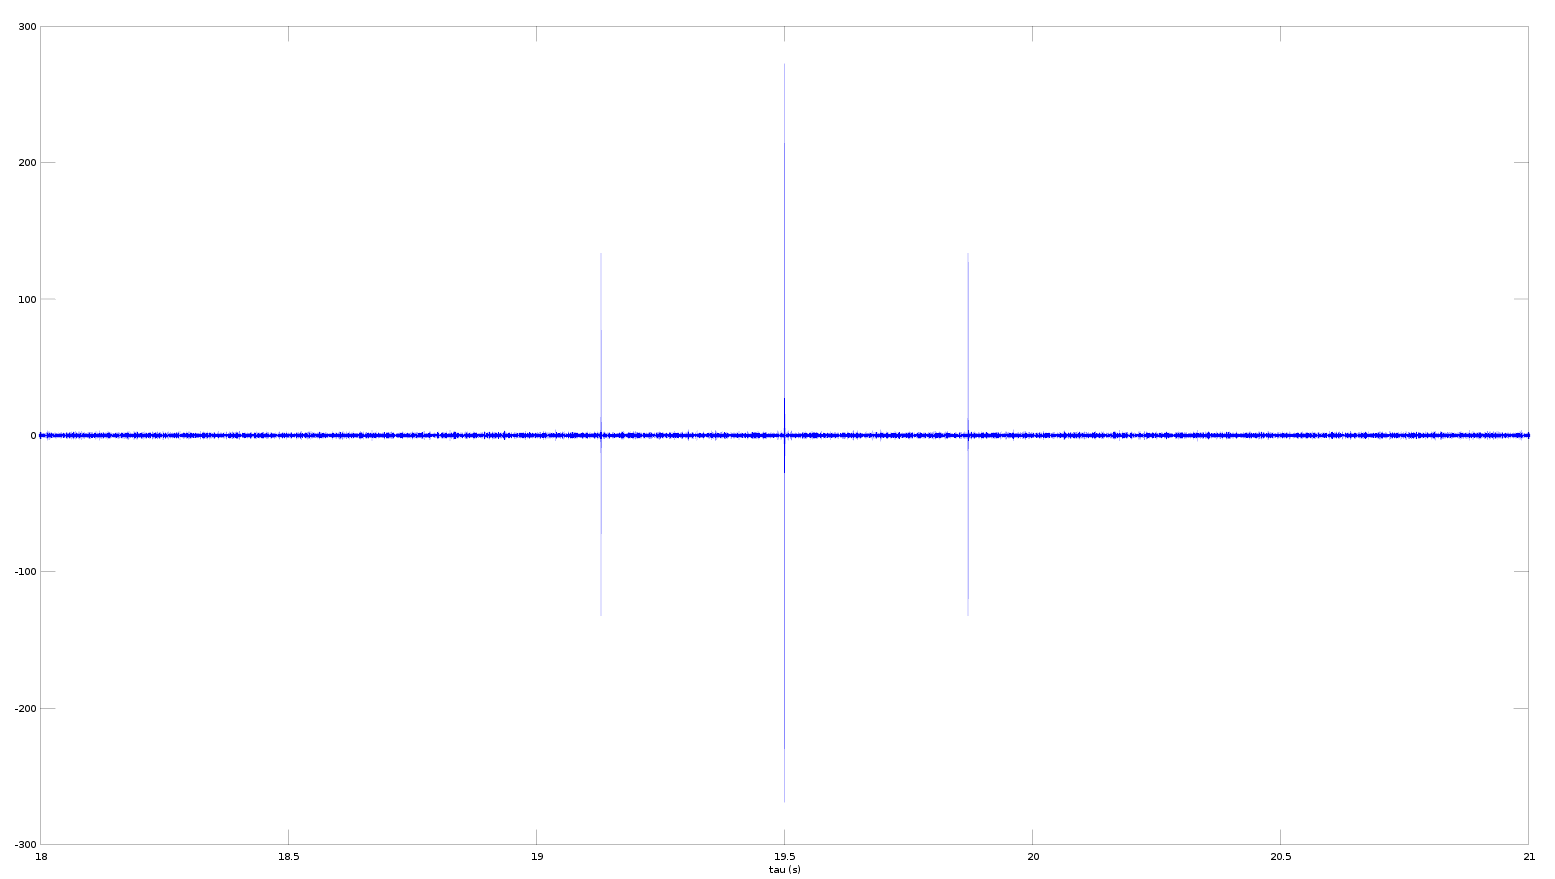
\includegraphics[keepaspectratio=true,width=\linewidth]{xCorr.png}  %skala och filnamn. 
  \end{center}
  \caption{Vitt brus x-korrelerat} %figurtext.
  \label{fig:xCorr}
\end{figure}
~\\
Mätningar ur figur \ref{fig:xCorr} ger att tidsfördröjningen är lika med $37 ms$. 

Då vi samplar med en frekvens av $400 000 Hz$ ges tidsfördröjningen i antal samples enligt nedan. 

\begin{gather}
samples = 0,37 \cdot 400 000 = 148 000
\label{equ:delaySamples}
\end{gather}
~\\
Eftersom ekot är fördröjt med $148 000$ samples är de första $148 000$ samplingarna av den utfiltrerade intressanta datan från frekvenstopp 1 utan eko. 

Med hjälp utav dessa $148 000$ första samples kan man sedan plocka bort ekot från nästkommande $148 000$ samples. Loopar man sedan igenom alla samples ($7 800 000$) filtrerar man helt bort ekot. 

Processen är inte helt enkel att uttrycka i ord - därav följer nedan utdrag ur den kod som finns i Appendix B. 

\begin{lstlisting}
% Filtrerar bort eko
% Anvander forsta 148 000 samples for att ta bort ekot som kommer sen.
nrOfSamples = 148000;

filtered = zeros(size(filterData1));
filtered(1:nrOfSamples) = filterData1(1:nrOfSamples);

for i = 0 : 50

temp1 = filtered((1+nrOfSamples*i):(nrOfSamples + nrOfSamples*i));
temp2 = filterData1((nrOfSamples+1+nrOfSamples*i):(i+2)*nrOfSamples);

filtered((nrOfSamples+1+nrOfSamples*i):(i+2)*nrOfSamples) = temp2 - 0.9*temp1;

end
\end{lstlisting}
~\\
Där filterData1 är den filtrerade signalen innehållandess frekvenstopp 1. 

\newpage

\subsection{I-/Q-demodulation}

För att demodulera signalen används principer som beskrivs av Erik G. Larsson (2014). I- och Q-komponenter ges enligt nedan: 

\begin{gather}
x_{I}(t) = \Large{H}\{2x(t)\cos{(2{\pi}f_{c}t + \theta)}\} \\
x_{Q}(t) = -\Large{H}\{2x(t)\sin{(2{\pi}f_{c}t + \theta)}\}
\label{equ:iq}
\end{gather}

Där $\theta$ är fasförskjutningen. Fasförskjutningen har tyvärr testats fram då möjligt område för den är relativt litet, $[0,\frac{\pi}{2}]$, och det vad undertecknad vet ej finns något sätt att entydigt bestämma fasförskjutningen. 


% -------- Slutsatser ------------

\newpage
\section{Resultat och slutsats}

Först spelas två melodier - varav en blinka lilla stjärna. Sedan hörs ordsspråket ''Man kan inte både ha kakan och äta den''.

% -------- Appendix ---------------

\newpage
\section{Källförteckning}

Larsson, Erik G, 2014. \textit{Signals, Information and Communications}. Draft 11342. Linköping. LiU-Press.


% -------- Appendix ---------------

\newpage
\appendix
\pagestyle{empty}
\newgeometry{left=2cm,right=2cm,bottom=2cm,top=2cm}
\section{Filtrerade signaler}

\begin{figure}[htp]
  \begin{center}
  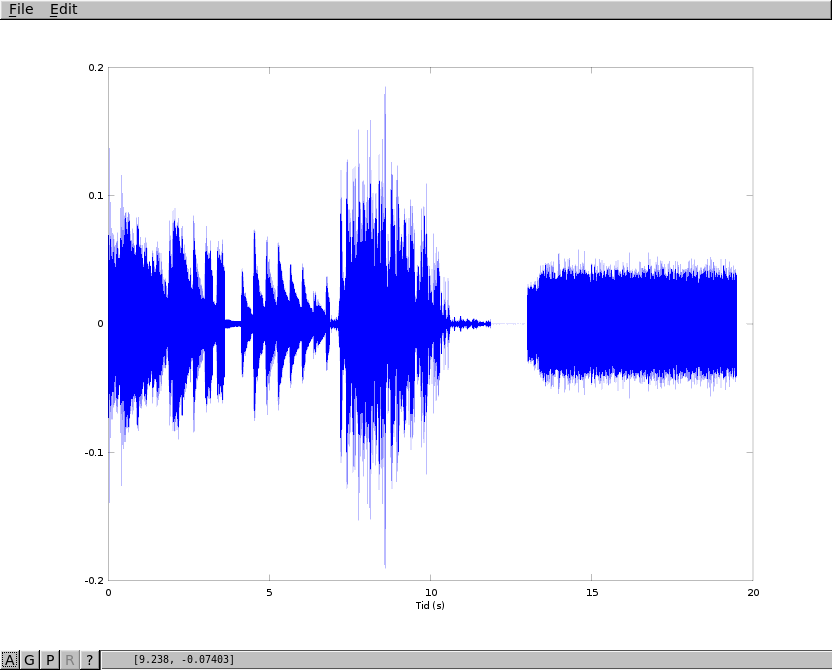
\includegraphics[keepaspectratio=true,width=\linewidth]{topp1_filter.png}  %skala och filnamn. 
  \end{center}
  \caption{Frekvenstopp 1 filtrerad} %figurtext.
  \label{fig:topp1_filter}
\end{figure}

\begin{figure}[htp]
  \begin{center}
  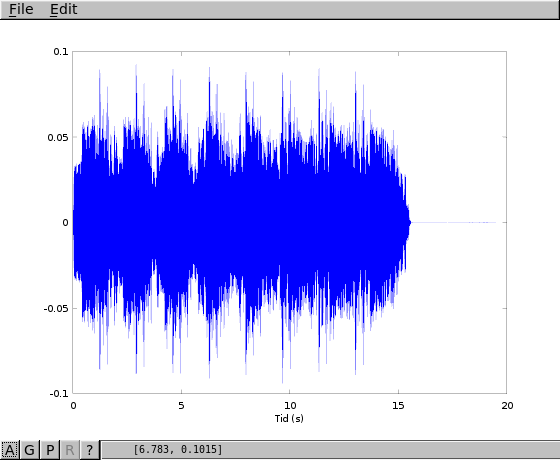
\includegraphics[keepaspectratio=true,width=\linewidth]{topp2_filter.png}  %skala och filnamn. 
  \end{center}
  \caption{Frekvenstopp 2 filtrerad} %figurtext.
  \label{fig:topp2_filter}
\end{figure}

\begin{figure}[htp]
  \begin{center}
  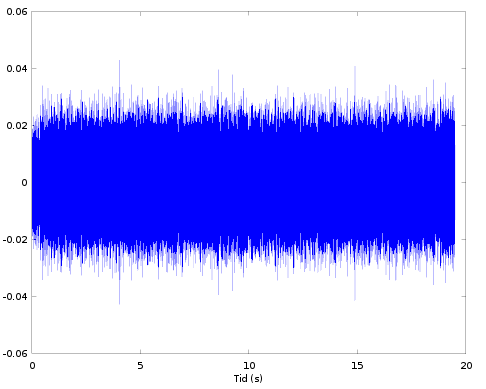
\includegraphics[keepaspectratio=true,width=\linewidth]{topp3_filter.png}  %skala och filnamn. 
  \end{center}
  \caption{Frekvenstopp 1 filtrerad} %figurtext.
  \label{fig:topp3_filter}
\end{figure}

\newpage
\section{Kod för GNU Octave}

\lstinputlisting{tsks10.m}

\end{document}